\documentclass{article}

\renewcommand{\labelenumii}{\theenumii}
\renewcommand{\theenumii}{\theenumi.\arabic{enumii}.}

\usepackage{graphicx}
\usepackage{hyperref} %might be better to uncomment this
\usepackage{subfig}
\usepackage{algpseudocode}
\usepackage{algorithm}

% Used for displaying a sample figure. If possible, figure files should
% be included in EPS format.
%
% If you use the hyperref package, please uncomment the following line
% to display URLs in blue roman font according to Springer's eBook style:
\renewcommand\UrlFont{\color{blue}\rmfamily}

\begin{document}
%
%\title{Contribution Title\thanks{Supported by organization x.}}
\title{[SCIR] Raporty 1-3}
%
%\titlerunning{very very very }
% If the paper title is too long for the running head, you can set
% an abbreviated paper title here

\author{Bartłomiej Mastej}
%
%
%
\maketitle              % typeset the header of the contribution
%
%
%
%
\section{Raport 1}
\subsection{Cel projektu}
Celem projektu jest stworzenie stacji pogodowej, która będzie zbierała dane za pomocą zintegrowanego czujnika wilgotności i temperatury oraz danych z kamerki.
Dane z kamerki mają być wstępnie przetważane lokalnie (Edge computing), a następnie wysyłane do chumury, gdzie na podstawie danych historycznych oraz danych z czujnika wilgotności i temperatury będą analizowane dalej. Ma to na celu przewidywanie temperatury "rzeczywistej" np poprzez wykrywanie opadów/zachmórzenia.

W celu zrealizowani projektu została wybrana platforma Raspberry Pi 4 model B, gdyż zapewnia względnie dużą moc obliczeniową, wystarczającą do prowadzenia prostej analizy danych lokalnie. Ponadto posiada wbudowany moduł wifi, co ułatwia komunikację z chmurą.

Cała dokumentacjpa do projektu znajduje się na GitHub'ie: \url{https://github.com/bartoszlomiej/weather-forecaster}.

\subsection{Schemat i części}
\begin{figure}
  %width=\textwidth
  \centering
  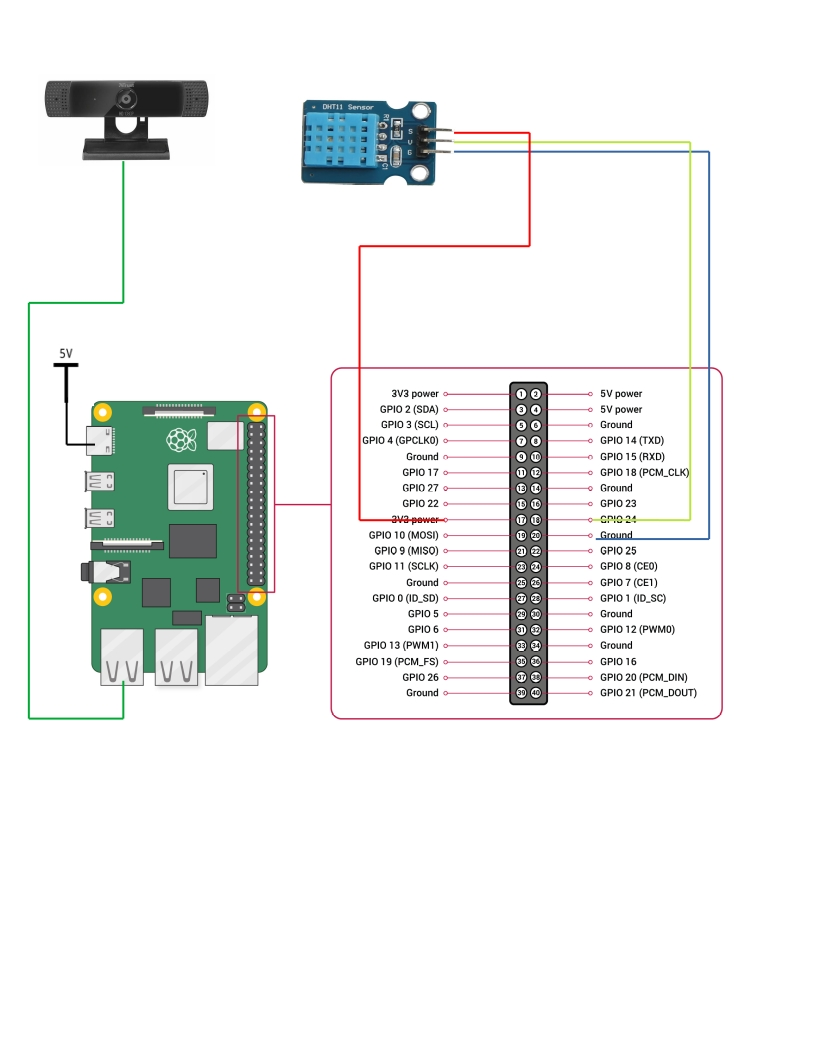
\includegraphics[width=\textwidth]{schemat.jpg}
\caption{Schemat podłączeń czujników do Raspberry Pi} \label{fig1}
\end{figure}
Użyte części:
\begin{enumerate}
\item Raspberry Pi 4 model B - platforma uruchmieniowa czujników oraz węzeł komunikacji,
\item DHT11 - czujnik temperatury i wilgotności,
\item TrustGX1160 - kamerka
\end{enumerate}

\subsection{Zbieranie danych z czujników}
\subsubsection{Konfiguracja Raspberry Pi}
Jako, że na Rasberry Pi został wgrany system operacyjny, komunikacja odbywa się po SSH. W celu skonfigurowania SSH należało dodać sieć wifi przy instalacji oraz dodać pusty plik $.ssh$ w folderze $/boot$ urządzenia. Pliki są wysyłane z komputera do Raspberry poprzez scp (secure copy, działające na zasadzie ssh). Potrzebne biblioteki zostały pobrane poprzez narzędzie $PIP$ języka $Python$.
\subsubsection{Czujnik wilgotności i temperatury - DHT11}
Czujnik DHT11 jest cyfrowy. W celu zbierania danych została wykorzystane biblioteki do Python'a: $RPI$ oraz $dht11$. Pierwsza z nich odpowiada za wykorzystanie Pinów ogólnego użytku (GPIO - general purpuse input output) i została wykorzsytana do pobierania danych z czujnika na pin'ie nr. 24. Natomiast druga biblioteka umożliwia wykorzystanie wcześniej wybranego pin'u do obioru danych z czujnika.
\subsubsection{Kamerka TrustGX1160}
Do zczytywania danych z kamerki została wykorzystana biblioteka $OpenCV$. Za pomocą funkcji $VideoCapture(0)$ kamerka jest uruchomiana, następnie wykonywane jest zdjęcie za pomocą funkcji $read()$. Następnie zdjęcie zapisywane jest do pliku. W dalszym etapie prac planowane jest wykorzystanie zdjęcia do oszacowania warunków pogodowych związanych z nasłonecznieniem oraz zachmurzeniem. W tym celu koniecznym będzie wprowadzenia obliczeń na $raspberry pi$ (edge computing).
\newpage
\section{Raport 2}
\subsection{Konfiguracja węzła}
Wszelkie zmiany w projekcie są dostępne na GitHub'ie: \url{https://github.com/bartoszlomiej/weather-forecaster}.
Jako, że platformą uruchomieniową jest Rasbperry Pi 4 model B, zatem konfiguracja przesyłu danych poprzez WiFi nie była skomplikowana. Zostało to wskazane w raporcie 1.

Podsumowując:
\begin{enumerate}
\item Komunikacja Raspberry z chmurą oraz z komputerem odbywa się poprzez wbudowany moduł WiFi.
\item Komunikacja z komputerem odbywa sie poprzez protokuł $ssh$ do pełnej kontroli, oraz przez $scp$ do przesyłu plików.
\item Komunikacja z chmurą wykorzystuje protokół MQTT.
\item Chmura użyta w projekcie to $Thingspeak$.
\end{enumerate}

\subsection{Wstępna komunikacja z chmurą}
Do skonfigurowania połączenia z chmurą po stronie Raspberry Pi za pomocą protokołu MQTT została wykorzystana biblioteka $paho.mqtt$.
Za pomocą gotowego API należy wpisać wymagane dane - id kanału, dane uwierzytelniające klienta, port, nazwę hosta, socket.
Konfiguracja (bez danych uwierzytelniających - ze względów bezpieczeństwa) została zaprezentowana na Fig.~\ref{fig:1}.
\begin{figure}
  %width=\textwidth
  \centering
  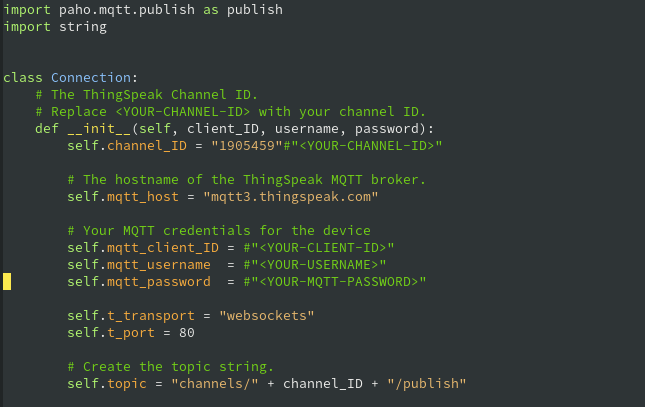
\includegraphics[width=\textwidth]{kod.png}
  \caption{Test odbierania danych w chmurze.} 
  \label{fig:1}    
\end{figure}

Wysyłanie danch z przygotowanym payload'em okazuje się bardzo proste - wystarczy użyć funkcji $publish$. Cała funkcja służąca do wysyłania payload'u na chmurę znajduę się na Fig.~\ref{fig:chm}.
\begin{figure}
  %width=\textwidth
  \centering
  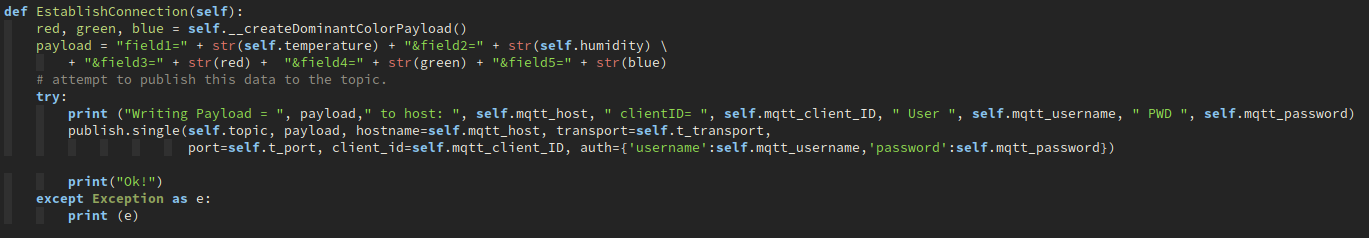
\includegraphics[width=\textwidth]{chm.png}
  \caption{Metoda publikacji danych po przez MQTT.}
  \label{fig:chm}    
\end{figure}

Po stronie chmury należy udostępnić dane konfiguracyjne MQTT (id klienta, nazwę użytkownika, hasło). Na Fig.~\ref{fig:2} zostało zaprezentowane prawidłowe odbieranie danych z raspberry pi. Jednakże, zamiast danych z czujników zostały wykorzystane parametry procesora (w celach testowych).
\begin{figure}
  %width=\textwidth
  \centering
  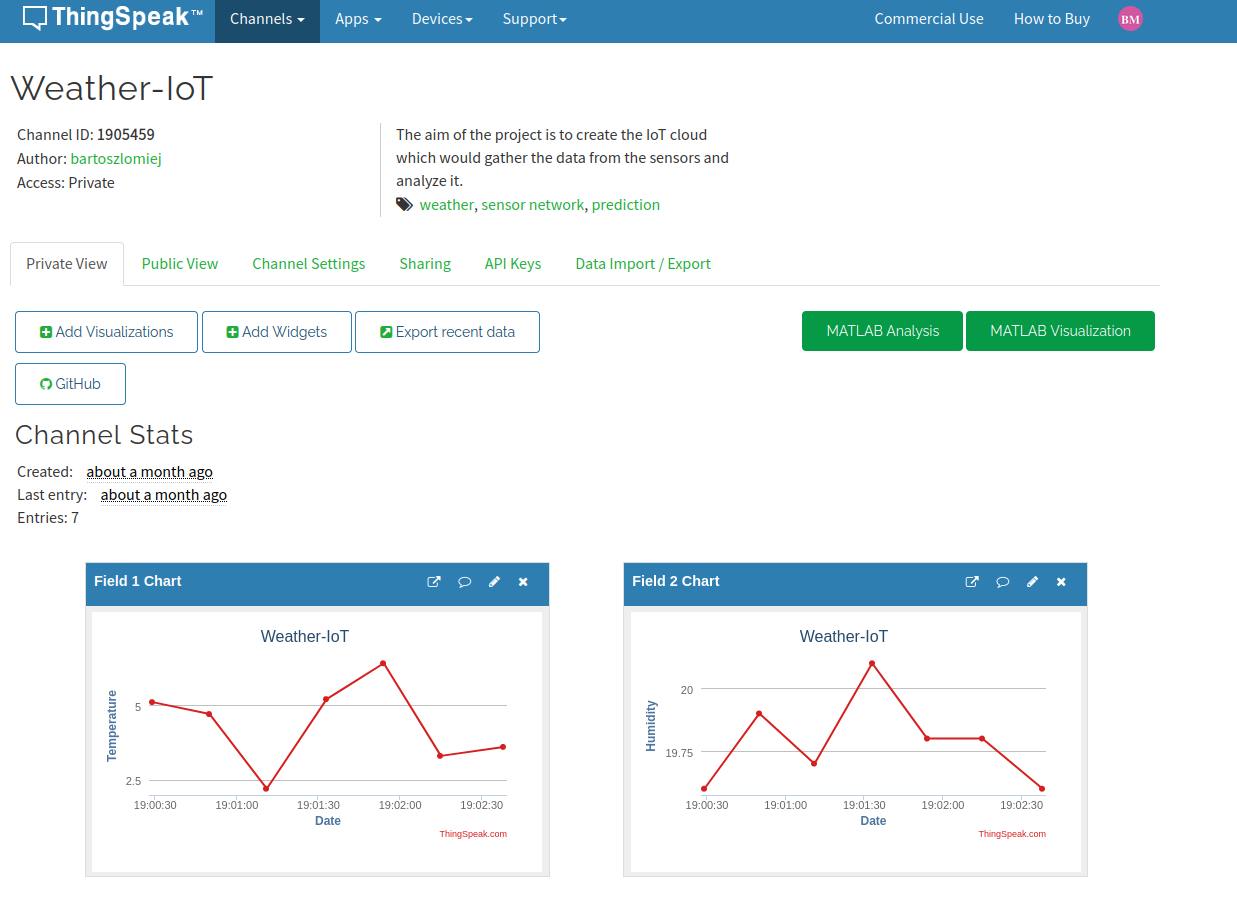
\includegraphics[width=\textwidth]{chumra.png}
  \caption{Test odbierania danych w chmurze.}
  \label{fig:2}    
\end{figure}
\subsection{Parallelizm zbierania danych - multithreading}
W celu wykonywania pomiarów z czujnika jednocześnie został wprowadzony multithreading z wykorzystaniem biblioteki $threading$. Za jego pomocą każdy z czujników zbiera dane jednocześnie. Przed ich ujendoliceniem następuje synchronizaca wątków.

W przyszłości ma to na celu jednoczesne prztwarzania obrazu, zbierania danych z czujników jak i ich wysyłania jeśli chwilami będzie to konieczne. Jednakże, zostanie to rozważone ze względu na optymalizację poboru mocy.
\newpage
\section{Raport 3}
\subsection{Multithreading}
Został kontynuowany pomysł z poprzedniego raportu - dane z czujników są pobierane na dwóch osobnych wątkach. Wynika to z faktu, iż pomiar temperatury i wilgotności pobiera wiele wartości w czasie i je uśrednia w celu zgromadzenia bardziej wiarygodnych pomiarów. Natomiast dane z kamery są przetwarzane co jest niestety względnie czasochłonne. Dzięki zrównolegleniu operacji dane z obu czujników wykonują się jednocześnie co umożliwia zwiększenie częstotliwości pobieranych danych. Dodatkowym atutem jest możliwość zwiększenia obliczeń na krawędzi chmury utrzymując stałą częstotliwość wysyłania danych do chmury. Zostały stworzone wątki zwracające wartości ($ReturnValueThread$). Kod równoległego pobierania danych z czujników zaprezentowany jest na Fig.~\ref{fig:watki}. Wspomniany wcześniej $ReturnValueThread$ znajduje się na Fig.~\ref{fig:ret}.
  \begin{figure}
    %width=\textwidth
  \centering
  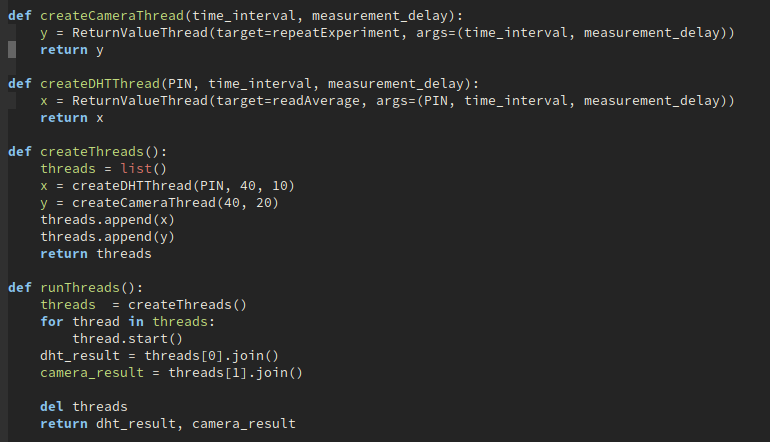
\includegraphics[width=\textwidth]{watki.png}
  \caption{Wielowątkowe gromadzenie danych.} \label{fig:watki}    
  \end{figure}

  \begin{figure}
    %width=\textwidth
  \centering
  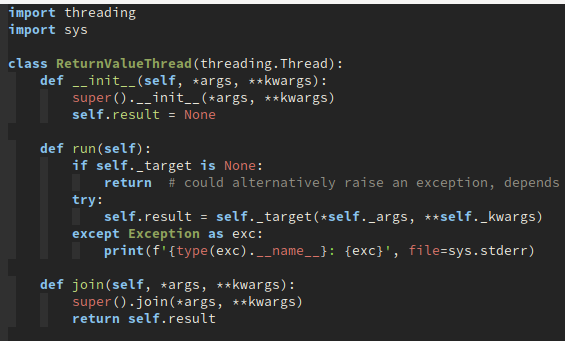
\includegraphics[width=\textwidth]{return.png}
  \caption{Return Value Thread.} \label{fig:ret}    
\end{figure}  

\subsection{Wczytywanie danych konfiguracyjnych MQTT}
W celach zapewnienia bezpieczeństwa danych konfiguracyjnych został utworzony specjalny plik $config.conf$, który nie jest udostępniany na repozytorium github. Znajduje się w nim najważniejsze dane autoryzacyjne dotyczące protokołu MQTT: $client\textunderscore ID$, $username$, $password$. Została przygotowana metoda w klasie $Connections$ służąca do parsowania danych (Fig.~\ref{fig:conf}).
  \begin{figure}
    %width=\textwidth
  \centering
  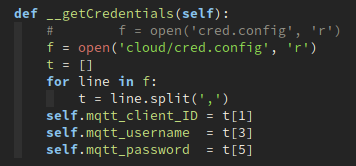
\includegraphics[scale = 1]{get_credentials.png}
  \caption{Parsowanie danych konfiguracyjnych.} \label{fig:conf}    
\end{figure}

\subsection{Przygotowanie danych z kamery}
Jako, że Thingspeak w wersji darmowej nie pozwala na wysyłanie zdjęć, koniecznym było dokonania obróbki danych na krawędzi (edge computing). Za wartościową wartość został uznany kolor dominujący na obrazie. Z założenia kamera nie zmienia swojej pozycji, dlatego jedyne co będzie się zmieniało na kamerze to kolory. Czyli dominujący kolor za dnia powinien być bardziej jasny, natomiast w nocy powininen być on niemalże czarny. Dodatkowo da się w ten sposób określić poziom zachmurzenia/nasłonecznienia, gdyż kolor dominujący będzie ulegał zmianą w czasie.

W celu znalezienia koloru dominującego został użyty algorytm klastrujący $kmeans$. Posiadając obraz w formacie $png$ możliwym jest odczytanie wartości RGB dla każdego piksela. Algorytm łączy podobne kolory w klastry, a następnie wskazuje ich centra - są to kolory dominujące w obrazie. Została użyta biblioteka $scipy.cluster.vq$ implementująca algorytm $kmeans$. Implementacja została pokazana na Fig.~\ref{fig:dom}. Warto zauważyć, że w celu uzyskania data frame wykorzystywana jest biblioteka $pandas$. Dodatkowo, pierwotnie odbyły się liczne próby implementacji z użyciem biblioteki $sklearn.cluster$, niestety na platformie $raspberry pi 4$ nie było to możliwe, gdyż platforma działa w architekturze $ARM$ i biblioteka nie została do niej dopasowana.

\begin{figure}
    %width=\textwidth
  \centering
  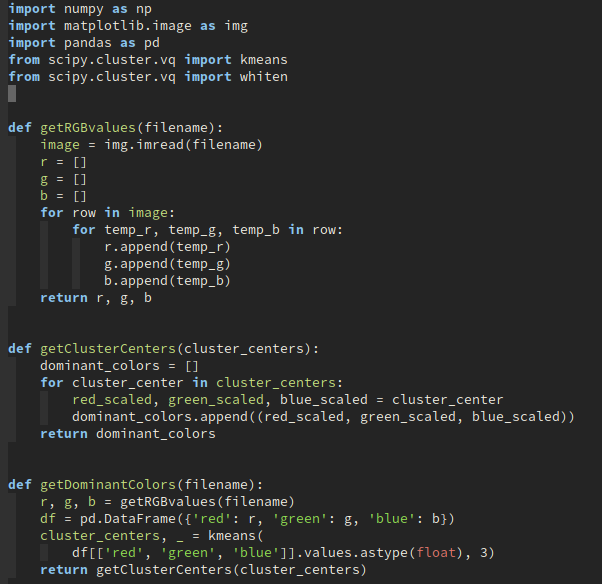
\includegraphics[scale = 1]{dominant.png}
  \caption{Otrzymywanie koloru dominującego z obrazu.} \label{fig:dom}    
\end{figure}

Chmura (Thingspeak) nie ułatwia wysyłania wielu danych, dlatego też zostało wprowadzone ograniczenie tylko do jednego koloru dominującego.

\subsection{Przygotowanie danych z czujnika DHT11}
W celu zwiększenia wiarygodności pomiarów zostało postanowione, aby liczyć średnią z wielu pomiarów. Zostało to oparte czasowo, aby pomiary były dokonywane w skończonym czasie. W tym celu został zaimplementowany timer. Jest to szczególnie ważne, gdyż czujnik często zwraca brak pomiaru (prawdopodobnie jest uszkodzony), dlatego też uzależnienie pomiarów od czasu pozwala nie szukać wartości w nieskończoność. Problem braku jakiejkolwiek wartości w danym czasie został rozwiązany w pętli głównej programu - w tak szczególnym wypadku pomiar jest powtarzany. Kod został zaprezentowany na Fig.~ \ref{fig:dht}. Zastosowane parametry $number\textunderscore of\textunderscore trials$ oraz $n$ służą do wskazania w logach urządzenia stosunku wszystkich prób pomiaru do udanych pomiarów.
\begin{figure}
    %width=\textwidth
  \centering
  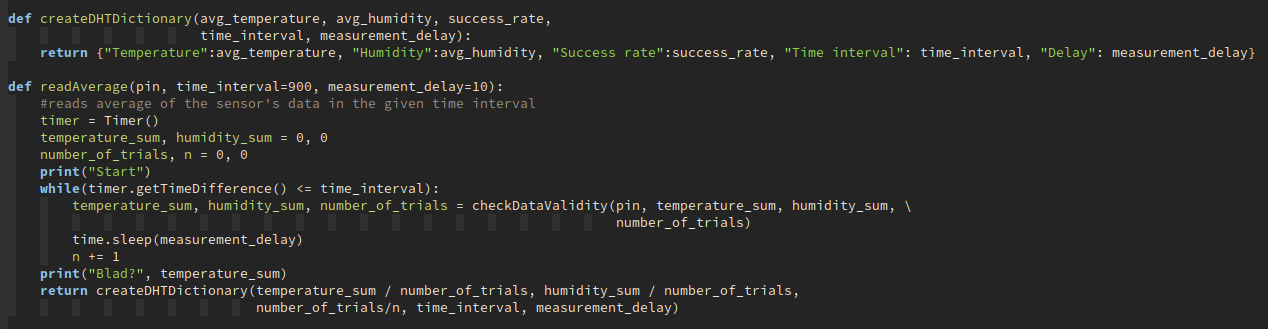
\includegraphics[width=\textwidth]{dht.png}
  \caption{Uśrednianie danych z czujnika DHT11.} \label{fig:dht}    
\end{figure}


\subsection{Otrzymywane dane w chmurze}
W celu zaprezentowania danych w przystępnej formie zostały zaprezenowane dwa rodzaje widgetów: wykresy oraz wyświetlacze liczb. Pierwsze z nich mają na celu pokazanie trendów i zależności w czasie. Natomiast drugie służą do zaprezentowania obecnych warunków pogodowych. Niestety, obecnie nie ma wskaźnika bezpośredniego naświetlenia (duże, małe, średnie), gdyż wymaga ono danych historycznych, które są jeszcze zbierane. Dane, które są trzymane w chmurze zostały pokazane na Fig.~\ref{fig:chm_2} oraz Fig.~\ref{fig:chm_1}.
\begin{figure}
    %width=\textwidth
  \centering
  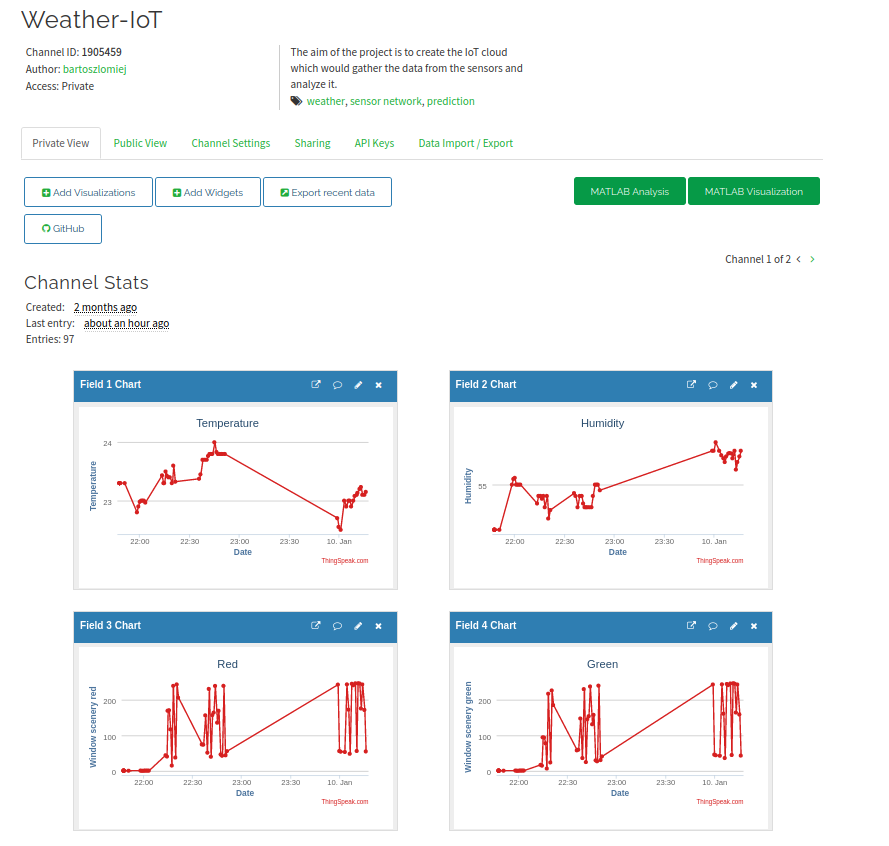
\includegraphics[width=\textwidth]{chmura_2.png}
  \caption{Dane prezentowane w chmurze - wykresy.} \label{fig:chm_2}    
\end{figure}

\begin{figure}
    %width=\textwidth
  \centering
  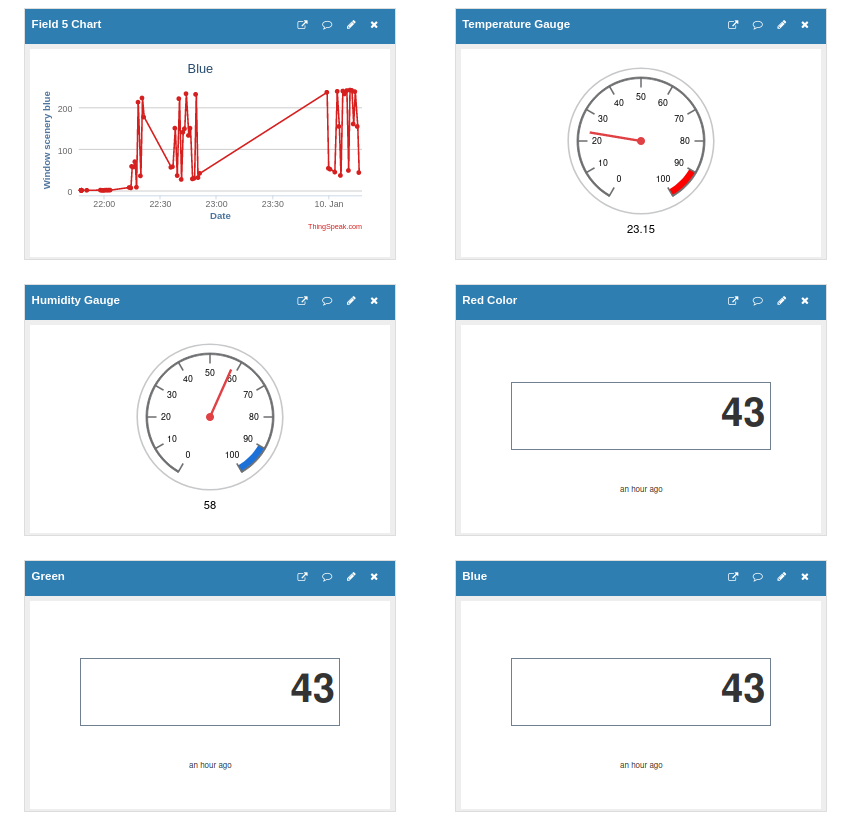
\includegraphics[width=\textwidth]{chmura_1.png}
  \caption{Dane prezentowane w chmurze - wyświetlacze liczb.} \label{fig:chm_1}    
\end{figure}


\end{document}
